\documentclass[11pt]{article}
\usepackage[margin=1in]{geometry}
\usepackage{amsmath,amssymb,amsthm,fontspec,fancyvrb,tikz}
\usepackage{unicode-math}
\usepackage[title]{appendix}
\setmonofont{JuliaMono}[Scale=0.76]
\usepackage[colorlinks=true,linkcolor=blue,citecolor=blue,urlcolor=blue]{hyperref}
\hypersetup{pdftitle={Relations among cycle invariants of a three-armed quiver},pdfauthor={P. Graham}}
\newtheorem{theorem}{Theorem}
\newtheorem{lemma}[theorem]{Lemma}
\newtheorem{corollary}[theorem]{Corollary}
\theoremstyle{remark}
\newtheorem{remark}[theorem]{Remark}
\newcommand{\CC}{\mathbb C}
\DeclareMathOperator{\Frac}{Frac}
\title{Relations among cycle invariants of a three-armed quiver}
\author{P. Graham\\ \small\url{https://orcid.org/0009-0007-8493-1505}}
\date{October 27, 2026}
\begin{document}
\maketitle
\begin{abstract}
Join two vertices by three paths, each with at least two edges, and give
each edge an arrow in each direction, with variables $d_{ij},u_{ij}$.
Put $D_i=\prod_jd_{ij}$ and $U_i=\prod_ju_{ij}$, and impose
$D_1-D_2+D_3=0$. Put $v_{ij}=d_{ij}u_{ij}$ and
$A=\prod_jv_{1j}$, $B=\prod_jv_{2j}$, $C=\prod_jv_{3j}$.
Under independent rescalings at the vertices, the ring of invariant
polynomial functions over $\CC$ has presentation
\[
 \CC[v_{ij},w_1,w_2,w_3]\big/I_2\!\begin{pmatrix}
 w_2&w_3&B\\ A&w_3+C&w_1
 \end{pmatrix}.
\]
Here $(w_1,w_2,w_3)=(D_1U_2,D_2U_1,-D_2U_3)$, and $I_2$ denotes the ideal
of $2\times2$ minors. Makonzi proved that these elements generate the
invariant ring. We prove that the minors generate all their relations,
with the corrected all-edge indexing of Remark~\ref{rem:versions},
establishing the kernel formulation of Makonzi's conjecture.
The key step is a specialization to
a rational function field that proves independence of normal forms.
Lean checks the kernel equality over $\CC$ for every triple of path
lengths at least two.
\end{abstract}

\noindent 2020 \emph{Mathematics Subject Classification}: 13A50, 13C40.\\
\emph{Keywords}: invariant ring, quiver, determinantal ideal, Lean.

\section{Introduction}
We prove the determinantal kernel presentation in Makonzi's
Conjecture 5.2 for a doubled three-armed quiver \cite{Makonzi}.
Fix integers $p_1,p_2,p_3\ge2$. For $i=1,2,3$ and $1\le j\le p_i$,
let $d_{ij},u_{ij},v_{ij}$ be indeterminates and put
\[
 D_i=\prod_jd_{ij},\qquad U_i=\prod_ju_{ij},\qquad
 P=\CC[v_{ij}],\qquad H=\CC[d_{ij},u_{ij}]/(D_1-D_2+D_3).
\]
We also write $D_i,U_i$ for their images in $H$.
Set $S=P[w_1,w_2,w_3]$, and define the $\CC$-algebra map $\Phi:S\to H$ by
\[
 (w_1,w_2,w_3)\longmapsto(D_1U_2,D_2U_1,-D_2U_3),\qquad
 v_{ij}\longmapsto d_{ij}u_{ij}.
\]
Write
$A=\prod_jv_{1j}$, $B=\prod_jv_{2j}$, $C=\prod_jv_{3j}$.
\begin{theorem}[Makonzi's Conjecture 5.2]\label{thm:main}
With the all-edge indexing $1\le j\le p_i$ of
Remark~\ref{rem:versions}, the kernel of $\Phi$ is the ideal $J$ generated
by the $2\times2$ minors of
\[
 \begin{pmatrix}w_2&w_3&B\\ A&w_3+C&w_1\end{pmatrix}.
\]
\end{theorem}
The new step is the kernel equality; generation and vanishing of the
minors are Makonzi's results. We first reduce polynomials modulo $J$ to
$P$-linear combinations of $1$ and powers of a single $w_i$.
The key choice is the specialization $\psi:H\to\Frac(P)(t)$ in the proof:
it sends $w_3$ to $t$, while the images of $w_1,w_2$ have poles at
$0,-C$, respectively. Comparing these poles proves independence of the
normal forms and hence $\ker\Phi\subseteq J$.

In Makonzi's quiver construction, take two vertices $s,q$ joined
by three paths (the arms), the $i$th having $p_i$ edges and
$p_i-1$ interior vertices.
Double each edge: $d_{ij}$ points from $s$ towards $q$ along the path,
and $u_{ij}$ points back.
Then $D_i,U_i$ are path products and $d_{ij}u_{ij}$ and $D_iU_k$ are
cycles. Figure~\ref{fig:quiver} depicts these paths schematically.
We take $p_i\ge2$, corresponding to three nonempty arms in the dual graph of \cite[\S2]{Makonzi}, where arm $i$ has $p_i-1$ vertices; the algebraic role of this assumption is discussed in Remark~\ref{rem:field}.
The ring $H$ is the quotient defined in \cite[Eq.~(3.1)]{Makonzi}.

Let $G$ be the torus with one copy of $\CC^*$ for each vertex of the
quiver. For $\mu=(\mu_v)_v\in G$ and an arrow $a$ with tail $\operatorname{tail}(a)$ and
head $\operatorname{head}(a)$, use Makonzi's action
\[
 \mu\cdot a=\mu_{\operatorname{tail}(a)}^{-1}a\mu_{\operatorname{head}(a)}.
\]
Each $D_i$ has weight $\mu_s^{-1}\mu_q$, so the defining ideal of $H$
is stable and the action descends to $H$.
We take the following generation result from Makonzi's Lemma 4.1,
Proposition 4.2, Lemma 4.3 and Proposition 5.1 \cite{Makonzi}:
\[
 H^G=\CC[d_{ij}u_{ij},D_1U_2,D_2U_1,-D_2U_3].
\]
Proposition 5.1 also proves that the three minors vanish.
For completeness, an invariant class in $H$ has a weight-zero polynomial
lift: decompose any lift into torus weights and discard the nonzero
weights, since the quotient map preserves weights. A weight-zero monomial
has equal incoming and outgoing multiplicities at every vertex. The
associated directed multigraph decomposes into directed cycles, by
successively following arrows until a vertex repeats and removing that
cycle. Thus cycle monomials generate the invariants. Makonzi's
Proposition 4.2 and Lemma 4.3 reduce these to the displayed finite list.
Write $\theta:S\to H^G$ for this surjective map and
$\iota:H^G\hookrightarrow H$ for inclusion. Then $\Phi=\iota\circ\theta$,
so $\ker\Phi=\ker\theta$.
Conjecture 5.2 asserts precisely that $\ker\theta$ is the ideal generated
by the $2\times2$ minors of that matrix. Theorem~\ref{thm:main} therefore gives:
\begin{corollary}\label{cor:invariants}
The map $\theta$ induces an isomorphism $S/J\cong H^G$.
\end{corollary}

\begin{remark}[Source conventions]\label{rem:versions}
We use the published kernel formulation. ArXiv v1 instead states:
``The ring homomorphism $\varphi$ is an isomorphism''
\cite[Conjecture 5.2]{MakonziV1}.
That map is unquotiented; the nonzero minor relations prevent its injectivity. ArXiv v2 has the kernel
formulation \cite{MakonziV2}. The published equations
(3.1) and (5.1) are (3.A) and (5.A) in v2. The map printed in \S5.1
uses $1<j\le p_i$; we use $1\le j\le p_i$, as required by the
first-edge entries in the matrix and \S4.3.
\end{remark}

Setting all $v_{ij}=v$ in the matrix, hence
$(A,B,C)=(v^{p_1},v^{p_2},v^{p_3})$, gives the rational determinantal
surface singularity of \cite[\S1.2]{Makonzi}, whose minimal resolution has a
star-shaped dual graph. The conjecture concerns the ring before these identifications.

Bruns and Vetter's Theorems (2.7) and (2.16) give perfection and
resolutions for maximal-minor ideals under a grade hypothesis; their
Theorem (16.36) gives the Hilbert--Burch description when a quotient
has a two-step free resolution \cite{BV}.
Our normal forms instead give a $P$-basis of $S/J$ and embed it in a
field, proving both the kernel equality and the domain assertion.

Immediately after Conjecture 5.2, Makonzi writes that calculations in
Magma ``confirm this in small cases, but the Gr\"obner approach seems
hard in general'' \cite[p.~17, paragraph following Conjecture 5.2]{Makonzi}.
An analogous quasideterminantal presentation for reconstruction algebras
of type A (cyclic quotient singularities) is Makonzi's Theorem 1.1
\cite{TypeA}. Reconstruction algebras and their resolution interpretation were developed
by Wemyss \cite[Definition 2.3, Theorems 3.24 and 4.5]{WemyssA};
the star-shaped algebra in \cite[\S2]{Makonzi} follows the double-quiver
presentation of Iyama and Wemyss \cite[Theorem 5.7]{IW}.
Wahl relates determinantal rational surface singularities to
$2\times(e-1)$ matrices and their exceptional curves
\cite[Proposition 3.2 and Theorem 3.4]{Wahl}.
Craw and Yamagishi give general trace generators and relation ideals for
quiver invariant rings \cite[Theorems 1.1 and 4.3]{CY}.
Their relation ideal lies in the invariant ring of the unconstrained
quiver. Here we give the three defining relations in Makonzi's specified
polynomial generators.


\begin{figure}[ht]
\centering
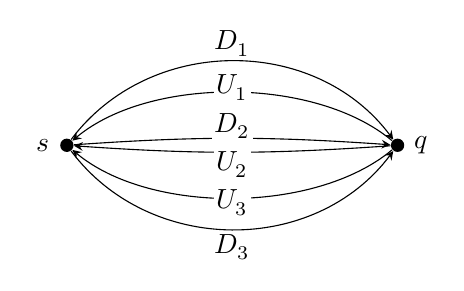
\begin{tikzpicture}[>=stealth,scale=0.7]
\node[circle,fill,inner sep=1.7pt,label=left:$s$] (s) at (-3,0) {};
\node[circle,fill,inner sep=1.7pt,label=right:$q$] (q) at (3,0) {};
\draw[->] (s) .. controls (-1.5,2) and (1.5,2) .. (q);
\draw[->] (q) .. controls (1.5,1.25) and (-1.5,1.25) .. (s);
\draw[->] (s) to[bend left=4] (q);
\draw[->] (q) to[bend left=4] (s);
\draw[->] (s) .. controls (-1.5,-2) and (1.5,-2) .. (q);
\draw[->] (q) .. controls (1.5,-1.25) and (-1.5,-1.25) .. (s);
\foreach \a/\y in {D_1/1.85,U_1/1.05,D_2/0.35,U_2/-0.35,U_3/-1.05,D_3/-1.85}
  \node[fill=white,inner sep=1pt] at (0,\y) {$\a$};
\end{tikzpicture}
\caption{Each pair of curves abbreviates a path of $p_i$ edges and its
reverse. The $p_i-1$ interior vertices of each path are suppressed;
$D_i,U_i$ denote products along the entire paths.}\label{fig:quiver}
\end{figure}

This work has not yet been reviewed by experts.
The proofs, the Lean formalization and the text were produced by AI models
(from OpenAI and Anthropic), working under the author's direction.

\section{Proof of Theorem~\ref{thm:main}}
The three minors give, modulo $J$,
\begin{equation}\label{eq:reduction}
 w_1w_2=AB,\qquad w_1w_3=Bw_3+BC,\qquad w_2w_3=Aw_3-Cw_2.
\end{equation}
We first find normal forms over $P$, then prove their uniqueness after
mapping $H$ to a rational function field. This gives the inclusion
$\ker\Phi\subseteq J$.

\begin{lemma}\label{lem:normal}
$S/J$ is generated as a $P$-module by
$1,w_1^n,w_2^n,w_3^n$ for $n\ge1$.
\end{lemma}
\begin{proof}
For a monomial involving at least two of $w_1,w_2,w_3$, apply the relevant
identity in \eqref{eq:reduction}. Each resulting monomial has smaller total
degree in $w_1,w_2,w_3$. Degree induction gives elements of $P$ or powers of a single $w_i$;
linearity gives the assertion, with coefficients in $P$.
\end{proof}

\begin{lemma}\label{lem:independent}
For a field $K$, an indeterminate $t$ and nonzero $\alpha,\beta,\gamma\in K$, the elements
\[
 1,\quad \left(\frac{\beta(t+\gamma)}t\right)^n,\quad
 \left(\frac{\alpha t}{t+\gamma}\right)^n,\quad t^n\qquad(n\ge1)
\]
of the rational function field $K(t)$ are linearly independent over $K$.
\end{lemma}
\begin{proof}
If the family $(\beta(t+\gamma)/t)^n$ has a nonzero coefficient in a finite relation, let
$m\ge1$ be the largest exponent whose coefficient $a_m$ is nonzero.
After multiplying by $t^m$, all terms are regular at $t=0$ since $\gamma\ne0$.
All vanish there except the $m$th power of the first family, which
contributes $a_m(\beta\gamma)^m\ne0$, a contradiction. Thus every coefficient in
that family is zero. Apply the same argument to $(\alpha t/(t+\gamma))^n$:
if $b_m$ is its highest nonzero coefficient, multiplication by $(t+\gamma)^m$
and evaluation at $t=-\gamma$ leave only $b_m(-\alpha\gamma)^m\ne0$, again a contradiction.
The remaining relation is a polynomial in $t$; all its coefficients
vanish.
\end{proof}

\begin{proof}[Proof of Theorem~\ref{thm:main}]
The relation $D_1-D_2+D_3=0$ gives
$\Phi(w_3+C)=-D_1U_3$, so the three minors vanish under $\Phi$. Hence
$J\subseteq\ker\Phi$, as also proved in \cite[Proposition 5.1]{Makonzi}.
For the reverse inclusion, take $K=\Frac(P)$, with the $v_{ij}$ algebraically independent, and let $t$ be transcendental over $K$.
Thus $A,B,C$ are nonzero in $K$.

Define a $\CC$-algebra homomorphism from $\CC[d_{ij},u_{ij}]$ to $K(t)$ by
\[
 d_{11}\mapsto(t+C)/t,\qquad d_{21}\mapsto1,\qquad
 d_{31}\mapsto-C/t,
\]
send the other $d_{ij}$ to $1$, and send
$u_{ij}$ to $v_{ij}$ divided by the image of $d_{ij}$.
Each image of $d_{ij}$ is nonzero. The relation $D_1-D_2+D_3$ maps to
$(t+C)/t-1-C/t=0$, so the map descends to $\psi:H\to K(t)$.
The images of $(U_1,U_2,U_3)$ are $(At/(t+C),B,-t)$.
Thus $\psi\circ\Phi$ satisfies
\[
 v_{ij}\mapsto v_{ij},\qquad
 (w_1,w_2,w_3)\mapsto\left(\frac{B(t+C)}t,\frac{At}{t+C},t\right).
\]
It suffices to show $\ker(\psi\circ\Phi)\subseteq J$, since $\ker\Phi\subseteq\ker(\psi\circ\Phi)$.
For $f\in\ker(\psi\circ\Phi)$, Lemma~\ref{lem:normal} gives $f-h\in J$ with
\[
 h=r+\sum_{n=1}^{N}(a_nw_1^n+b_nw_2^n+c_nw_3^n),
 \qquad r,a_n,b_n,c_n\in P.
\]
Since $J\subseteq\ker\Phi$, we have
$\psi\Phi(h)=0$. Apply Lemma~\ref{lem:independent} with
$(\alpha,\beta,\gamma)=(A,B,C)$ and the indeterminate $t$. Every coefficient vanishes
in $K$, hence in $P$ by the injection $P\hookrightarrow K$.
Thus $h=0$ and $f\in J$. Since $\psi\Phi(J)=0$, we have
$\ker(\psi\circ\Phi)=J$ and hence $\ker\Phi=J$.
\end{proof}

\begin{corollary}\label{cor:free}
The ring $S/J$ is a domain and a free $P$-module with basis
$1,w_1^n,w_2^n,w_3^n$ for $n\ge1$.
\end{corollary}
\begin{proof}
The map $\psi\Phi$ embeds $S/J$ into $K(t)$.
Lemma~\ref{lem:normal} gives spanning over $P$, and
Lemma~\ref{lem:independent} gives independence.
\end{proof}
In particular, $\operatorname{Spec}(S/J)\to\operatorname{Spec}P$ is flat,
since $S/J$ is a free $P$-module.

\begin{remark}\label{rem:field}
For the map $\Phi$ defined above, the same kernel equality holds over
any field $k$ for $p_i\ge1$. Indeed, with $P=k[v_{ij}]$, the monomials
$A,B,C$ are still nonzero, and Lemmas~\ref{lem:normal} and
\ref{lem:independent} apply in every characteristic.
The specialization assigns special values to $d_{11},d_{21},d_{31}$
and sends each $d_{ij}$ with $j>1$ to $1$; it sends every $u_{ij}$
to $v_{ij}$ divided by the chosen image of $d_{ij}$.
Thus all $v_{ij}$ are retained, and only the existence of the first
edge of each path is needed.
The invariant-ring interpretation above uses Makonzi's three nonempty
arms, with $p_i\ge2$.
\end{remark}

\section{Formal verification}
The main formal theorem is \texttt{Makonzi.kernel\_equality}:
\VerbatimInput[fontsize=\small,samepage=true]{../data/statement.lean}
The coefficient field in these definitions is $\CC$. The source of
\texttt{phi} is the polynomial ring $S$, and its target is the arrow
polynomial ring modulo $D_1-D_2+D_3$, namely $H$. Its variable images are
$v_{ij}\mapsto d_{ij}u_{ij}$ and
$(w_1,w_2,w_3)\mapsto(D_1U_2,D_2U_1,-D_2U_3)$.
The definition \texttt{minorIdeal} is the ideal of the three minors of
the matrix in Theorem~\ref{thm:main}, including its $w_3+C$ entry.
The arm and edge indices are shifted by one in Lean. Thus the displayed equality
is exactly $\ker\Phi=J$ for $p_i\ge2$.
Lean \cite{Lean4}, with Mathlib \cite{Mathlib}, checks both
containments, normal-form reduction and rational-function independence.
Makonzi's Lemma 4.1, Proposition 4.2, Lemma 4.3 and Proposition 5.1 supply the generation result
used in Corollary~\ref{cor:invariants}.
Corollary~\ref{cor:free} and Remark~\ref{rem:field} are not formalized.
The formalization and its checking guide, including the pinned versions
and axiom dependencies, are available at \cite{Supplement}.

\begin{thebibliography}{12}
\small\raggedright
\bibitem{Makonzi}
B. Makonzi, \emph{Deformations and Simultaneous Resolution of Determinantal
Surfaces}, The Quarterly Journal of Mathematics \textbf{76} (2025),
1355--1372. \url{https://doi.org/10.1093/qmath/haaf044}.
Statement locators refer to the 18-page Advance Access article,
published November 25, 2025.
\bibitem{MakonziV2}
B. Makonzi, \emph{Deformations and Simultaneous Resolution of Determinantal
Surfaces}, arXiv:2309.02982v2 (October 30, 2025).
\url{https://arxiv.org/abs/2309.02982v2}.
\bibitem{MakonziV1}
B. Makonzi, \emph{Deformations and Simulatenous Resolutions of Determinantal
Surfaces}, arXiv:2309.02982v1 (September 6, 2023).
\url{https://arxiv.org/abs/2309.02982v1}.
\bibitem{TypeA}
B. Makonzi, \emph{The Artin component and simultaneous resolution via
reconstruction algebras of type A}, Journal of Noncommutative Geometry
\textbf{18} (2024), 1229--1264. \url{https://doi.org/10.4171/jncg/552}.
\bibitem{IW}
O. Iyama and M. Wemyss, \emph{Weighted Projective Lines and Rational Surface
Singularities}, \'{E}pijournal de G\'eom\'etrie Alg\'ebrique \textbf{3} (2019),
article 13; published January 14, 2020.
\url{https://doi.org/10.46298/epiga.2020.volume3.4761}.
The journal-hosted PDF is also arXiv:1606.09445v3.
\bibitem{BV}
W. Bruns and U. Vetter, \emph{Determinantal Rings}, Lecture Notes in
Mathematics \textbf{1327}, Springer-Verlag, 1988.
\url{https://doi.org/10.1007/BFb0080378}.
\bibitem{WemyssA}
M. Wemyss, \emph{Reconstruction Algebras of Type A}, Transactions of the
American Mathematical Society \textbf{363} (2011), 3101--3132.
\url{https://arxiv.org/abs/0704.3693v4} (statement numbering).
\bibitem{Wahl}
J. M. Wahl, \emph{Equations defining rational singularities}, Annales
scientifiques de l'\'Ecole Normale Sup\'erieure (4) \textbf{10} (1977),
231--263. \url{https://doi.org/10.24033/asens.1326}.
\bibitem{CY}
A. Craw and R. Yamagishi, \emph{The Le Bruyn--Procesi theorem following
Lusztig}, arXiv:2312.08527v4 (November 14, 2025).
\url{https://arxiv.org/abs/2312.08527v4}.
\bibitem{Lean4}
L. de Moura and S. Ullrich, \emph{The Lean 4 Theorem Prover and Programming
Language}, Automated Deduction---CADE 28 (2021).
\url{https://doi.org/10.1007/978-3-030-79876-5_37}.
\bibitem{Mathlib}
The mathlib Community, \emph{The Lean Mathematical Library},
Certified Programs and Proofs (CPP 2020).
\url{https://doi.org/10.1145/3372885.3373824}.
\bibitem{Supplement}
P. Graham, \emph{Supplementary material for Relations among cycle invariants
of a three-armed quiver}, version 1 (2026).
\url{https://github.com/6/clank-lab/tree/makonzi-invariants-v1/results/makonzi-invariants}
\end{thebibliography}
\end{document}
